\chapter{Factor graphs and pose graphs}
\label{ch:posegraph}

The local bundle adjustment of Chapter~\ref{ch:ba} keeps the recent past
accurate and forgets the rest. To correct the accumulated drift we need
constraints that reach far back in time --- loop closures --- and a
problem small enough to re-solve over the whole trajectory every time
one arrives. A \emph{pose graph} is that problem: the keyframe poses
only, linked by relative-pose measurements. This chapter returns to the
factor graphs of Chapter~\ref{ch:slam} with the tools now available,
derives the Jacobians that pose graphs need (which takes us back to the
Lie theory of Chapter~\ref{ch:rigid}, on $\SE3$ this time), closes the
loops of our garden, and then studies the operation that every
long-running estimator performs and that is easy to get subtly wrong:
marginalisation.

\section{Factor graphs, once more}

\begin{definition}{Nonlinear factor graph}{nlfg}
A nonlinear factor graph has variables $\btheta=(\btheta_1,\dots,
\btheta_N)$, each on a vector space or a Lie group, and factors
$a\in\mathcal{F}$, each a function of a few variables $\btheta_a$ with a
residual $\vect{e}_a(\btheta_a)$ and an information matrix $\Omega_a$.
Its MAP estimate minimises $\tfrac12\sum_a\rho_a\bigl(\vect{e}_a\T
\Omega_a\vect{e}_a\bigr)$.
\end{definition}

Everything we have solved fits this mould: the linear problem of
Chapter~\ref{ch:slam}, calibration (Chapter~\ref{ch:nls}), bundle
adjustment (Chapter~\ref{ch:ba}). What differs from one problem to
another is the set of factor \emph{types} and the graph's shape. The
solution method is always Gauss--Newton or Levenberg--Marquardt, and its
cost is dominated by the factorisation of $H$, whose sparsity is the
graph (\cref{prop:sparsity}). Solving $H\vect\delta=-\vect{g}$ by
Cholesky is variable elimination, one variable at a time: each
elimination is the marginalisation of \cref{lem:schur} and connects the
eliminated variable's neighbours (\cref{prop:fillin}). The order of
elimination therefore decides how much fill-in is created; finding a good
order is NP-hard in general, but heuristics such as COLAMD do well, and
in bundle adjustment the obvious order --- points first --- is already
excellent (\cref{thm:schurba}). Libraries such as GTSAM and g2o are, at
heart, a catalogue of factor types plus this sparse elimination
machinery.

\section{Jacobians on $\SE3$}

A relative-pose factor compares two poses through a logarithm, so its
Jacobian requires the derivative of $\Log$ on $\SE3$, generalising
\cref{thm:jr}.

\begin{theorem}{Right Jacobian of $\SE3$}{jrse3}
Let $\ad(\bxi)=\bigl(\begin{smallmatrix}\hatop{\bphi}&\hatop{\brho}\\0&
\hatop{\bphi}\end{smallmatrix}\bigr)$ for $\bxi=(\brho,\bphi)$. Then
$\frac{d}{dt}\Exp(\bxi(t))=\Exp(\bxi)\,\hatop{(J_r(\bxi)\dot\bxi)}$ with
\begin{equation}\label{eq:jrse3}
J_r(\bxi)=\sum_{n\ge0}\frac{(-\ad\bxi)^n}{(n+1)!},\qquad
J_r(\bxi)^{-1}=\sum_{n\ge0}\frac{B_n}{n!}(-\ad\bxi)^n\quad
(\norm{\bphi}<2\pi),
\end{equation}
where $B_n$ are the Bernoulli numbers ($B_0=1$, $B_1=-\frac12$, $B_2=
\frac16$, $B_3=0$, $B_4=-\frac1{30}$, \dots). Consequently
$\Log(\Exp(\bxi)\Exp(\vect\delta))\approx\bxi+J_r(\bxi)^{-1}\vect\delta$.
\end{theorem}

\begin{proof}
\Cref{lem:dexp} holds for any matrix exponential, and gives, with
\cref{prop:adjoint},
\[
\Exp(-\bxi)\frac{d}{dt}\Exp(\bxi)=\int_0^1\Exp(-s\bxi)\hatop{\dot\bxi}
\Exp(s\bxi)\,ds=\int_0^1\hatop{\bigl(\Ad_{\Exp(-s\bxi)}\dot\bxi\bigr)}ds.
\] Next, $\Ad_{\Exp(t\bxi)}=\exp(t\ad\bxi)$: both
sides equal $I$ at $t=0$ and satisfy $\frac{d}{dt}M(t)=M(t)\ad\bxi$, the
left one because $\frac{d}{dt}\Exp(t\bxi)\hatop{\vect{y}}\Exp(-t\bxi)=
\Exp(t\bxi)[\hatop{\bxi},\hatop{\vect{y}}]\Exp(-t\bxi)$ and
$[\hatop{\bxi},\hatop{\vect{y}}]=\hatop{(\ad(\bxi)\vect{y})}$ (direct
computation, checked in the tests). Hence $J_r=\int_0^1e^{-s\ad\bxi}ds=
f(-\ad\bxi)$ with $f(z)=(e^z-1)/z=\sum_nz^n/(n+1)!$, an entire function.
The function $g(z)=z/(e^z-1)=\sum_nB_nz^n/n!$ is analytic for $|z|<2\pi$
and $fg=1$ there. The matrix $\ad\bxi$ is block triangular with diagonal
blocks $\hatop{\bphi}$, whose eigenvalues are $0$ and $\pm i\norm{\bphi}$
(Exercise~\ref{ex:2eig}); so if $\norm{\bphi}<2\pi$ the series $g(-\ad
\bxi)$ converges and $f(-\ad\bxi)\,g(-\ad\bxi)=I$. The last statement
follows as in the proof of \cref{thm:jr}.
\end{proof}

The rotation block of $J_r(\bxi)$ is the $\SO3$ right Jacobian of
\cref{thm:jr}; the series converge fast for the small residuals of a
pose graph near its optimum, and the code sums twenty terms.

\begin{proposition}{Relative-pose factor}{between}
Let $Z_{ij}$ measure $T_i^{-1}T_j$, and $\vect{e}_{ij}=\Log(Z_{ij}^{-1}
T_i^{-1}T_j)$. With right perturbations of $T_i$ and $T_j$,
\[
\frac{\partial\vect{e}_{ij}}{\partial\bxi_j}=J_r(\vect{e}_{ij})^{-1},
\qquad
\frac{\partial\vect{e}_{ij}}{\partial\bxi_i}=-J_r(\vect{e}_{ij})^{-1}
\Ad_{T_j^{-1}T_i}.
\]
\end{proposition}

\begin{proof}
Let $E=Z_{ij}^{-1}T_i^{-1}T_j$. Perturbing $T_j$ gives $E\Exp(\bxi_j)$,
and \cref{thm:jrse3} gives the first Jacobian. Perturbing $T_i$ gives
$Z_{ij}^{-1}\Exp(-\bxi_i)T_i^{-1}T_j=E\,(E^{-1}Z_{ij}^{-1})\Exp(-\bxi_i)
(E^{-1}Z_{ij}^{-1})^{-1}$, and $E^{-1}Z_{ij}^{-1}=T_j^{-1}T_i$; by
\cref{prop:adjoint} this is $E\Exp(-\Ad_{T_j^{-1}T_i}\bxi_i)$, and
\cref{thm:jrse3} again gives the second Jacobian.
\end{proof}

\section{Pose graphs and loop closures}

\begin{definition}{Pose graph}{posegraph}
A pose graph has one variable per keyframe pose $T_i\in\SE3$ and one
factor per relative-pose measurement $Z_{ij}$, with information
$\Omega_{ij}$: \emph{odometry} factors between consecutive keyframes,
from the VO, and \emph{loop-closure} factors between keyframes far apart
in time that see the same place. One pose is held fixed (gauge).
\end{definition}

A pose graph is what remains of bundle adjustment when the points are
marginalised out and each pair of keyframes' joint information is
summarised by a single relative-pose Gaussian. That summary throws
information away (the true marginal couples many keyframes at once, and
it is not Gaussian), which is why the result is usually refined
afterwards by a full BA, as ORB-SLAM does. But the pose graph has a few
hundred variables instead of tens of thousands, and solving it after
each loop closure takes a fraction of a second.

\paragraph{The garden.} We take the keyframes of the Chapter~\ref{ch:vo}
VO on the 60\,m mowing pattern, with their 36.5\,cm RMS drift, and add a
loop closure wherever two keyframes at least twenty keyframes apart see
at least thirty common structure landmarks. Recognising such places from
the images is the subject of Chapter~10; here the simulator tells us,
and the relative pose is measured with 2\,cm and $0.3^\circ$ of noise,
the accuracy of the PnP of Chapter~\ref{ch:vo}. The mowing pattern
produces 27 such loops, mostly between neighbouring rows that face the
same way and see the same fence, house and trees. Optimising the pose
graph brings the RMS error from 36.5\,cm to 3.5\,cm (\cref{fig:pgo}). For
the keyframes of the VO with local bundle adjustment, it goes from 4.2 to
3.0\,cm with 72 loops.

\begin{figure}[ht]
\centering
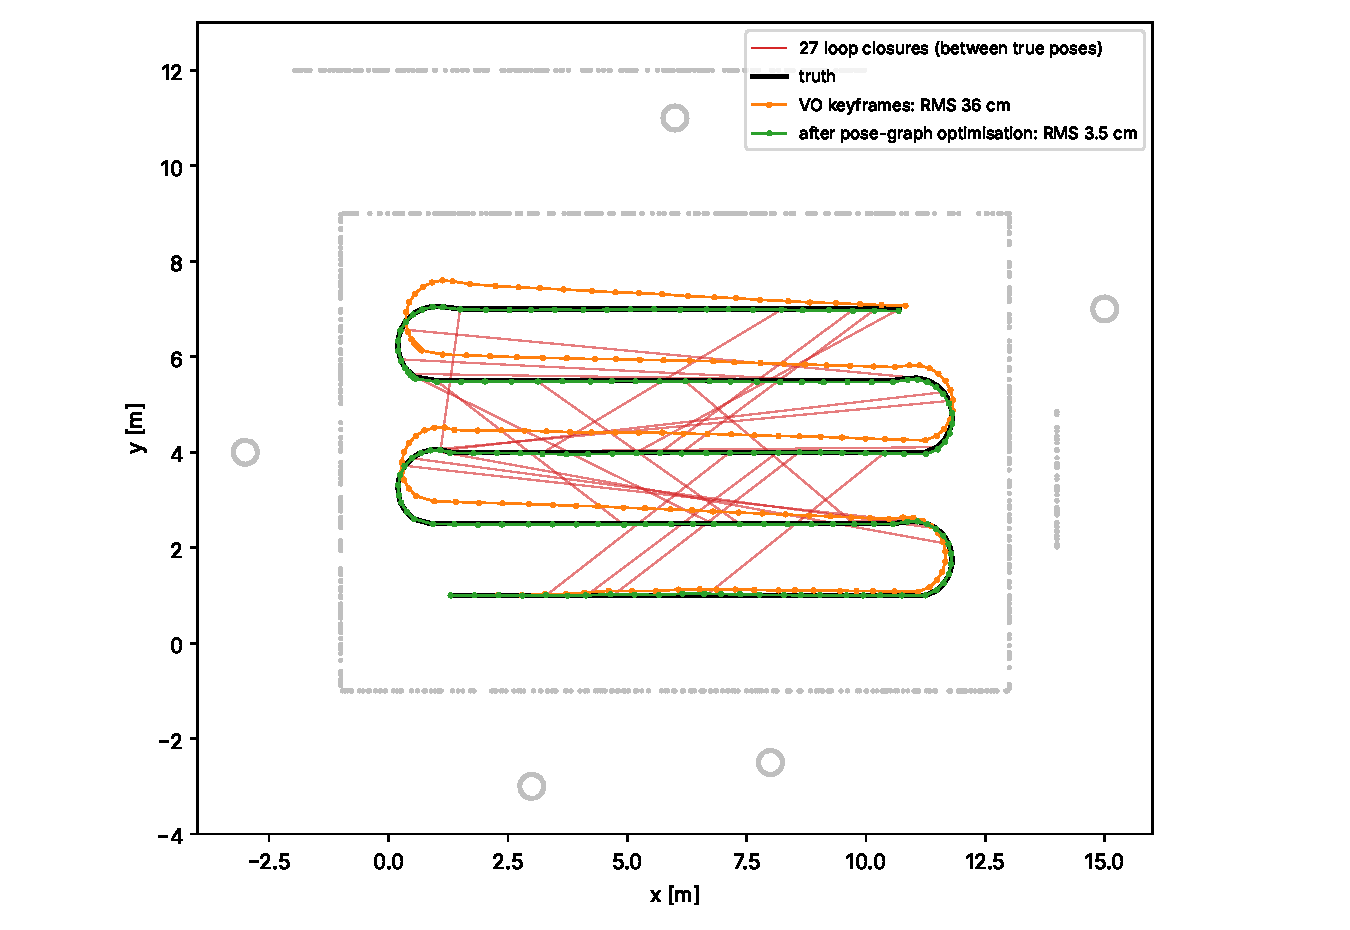
\includegraphics[width=0.85\linewidth]{figures/ch09_pgo.pdf}
\caption{Pose-graph optimisation of the 153 keyframes of the keyframe VO
of Chapter~\ref{ch:vo} (orange), with 27 loop closures (red, drawn
between the true positions) and odometry factors of standard deviation
2\,cm and $0.23^\circ$. Green: the optimised keyframes.}
\label{fig:pgo}
\end{figure}

\paragraph{How much to trust the odometry.} The information of the
odometry factors is a modelling choice with real consequences. The VO's
keyframe-to-keyframe errors have an empirical spread of 0.6\,cm and
$0.06^\circ$; using these as the factor's standard deviations gives a
worse result, 5.6\,cm, than inflating them by three or four (3.5\,cm).
The reason is that consecutive odometry errors are correlated --- the
same mis-triangulated map points bias several successive keyframes ---
whereas the factor graph treats them as independent, and so believes the
odometry too strongly. Covariances taken from the BA
(\cref{prop:bacov}) are optimistic for the same reason, and practical
systems inflate them.

\section{Robustness to wrong loops}
\label{sec:pgrobust}

A loop closure is a claim that two images show the same place. On a
lawn, where fence sections and rows look alike, some of these claims
will be wrong, and a single wrong loop closure entered as a Gaussian
factor bends the whole trajectory towards it (\cref{fig:pgrobust}): the
RMS error jumps from 3.5\,cm to over a metre. The remedies are the
robust kernels of Chapter~\ref{ch:nls}, applied per factor (a loop
factor is one block of six residuals), and their more elaborate
relatives: switchable constraints (Sünderhauf and Protzel) and dynamic
covariance scaling (Agarwal et al.), which add a weight variable per
loop, and graduated non-convexity (Yang et al.), which starts from a
convex problem and makes it progressively robust. A Cauchy kernel
already absorbs twenty wrong loops; its price is a slightly larger error
in the clean case, 4.3 instead of 3.5\,cm, because it also down-weights
the correct loops with the largest residuals.

\begin{figure}[ht]
\centering
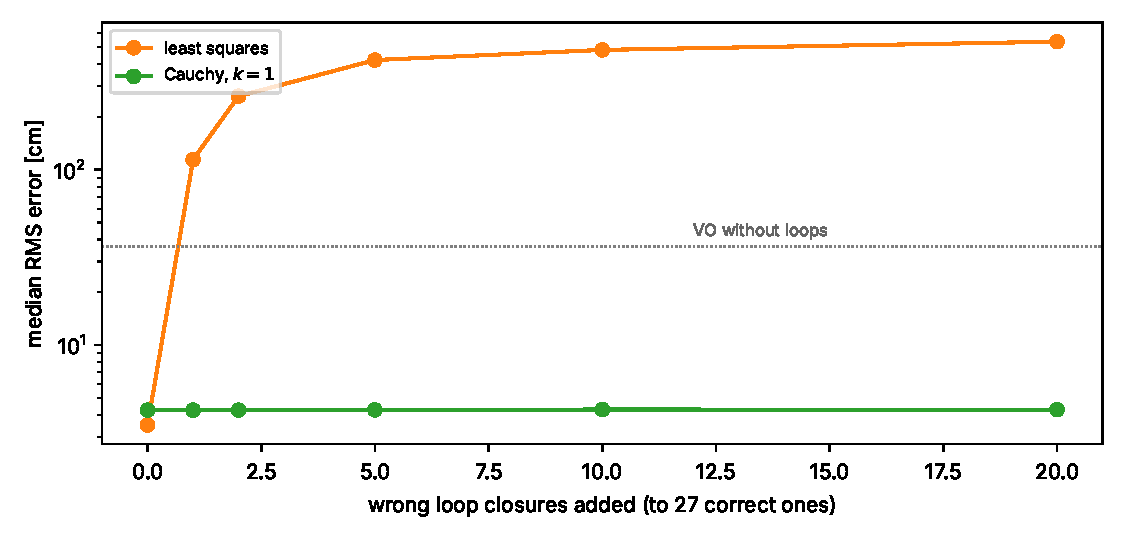
\includegraphics[width=0.8\linewidth]{figures/ch09_robust.pdf}
\caption{Adding wrong loop closures (random pairs of keyframes declared
to be within about 30\,cm and $3^\circ$ of each other) to the 27 correct
ones; median over 10 draws. Least squares is ruined by the first one;
the Cauchy kernel ignores them.}
\label{fig:pgrobust}
\end{figure}

\begin{inwords}
A robust kernel cannot tell a wrong loop from a correct loop that
disagrees with badly drifted odometry. With the overconfident odometry
of the previous section, the correct loops start with residuals of
eighteen standard deviations and the Cauchy kernel discards them too:
the error stays at 28\,cm (notebook, section~4). Robust estimation works
only together with an honest noise model, or with a schedule that
starts permissive. And it is no substitute for checking loop
candidates geometrically before they ever enter the graph (Chapter~10).
\end{inwords}

\section{Marginalisation}

A sliding-window estimator that runs for hours cannot keep every
variable, and simply dropping old variables (as our local BA does, by
fixing the oldest keyframe and discarding the rest) throws away their
information. The principled alternative is to marginalise them: replace
them, and all the factors that touch them, by a single Gaussian prior on
the variables they were connected to.

\begin{proposition}{Marginal prior}{margprior}
Linearise the factors that involve a set of variables $\btheta_d$ to be
removed, at the current estimate, and let $\begin{psmallmatrix}H_{kk}&
H_{kd}\\H_{dk}&H_{dd}\end{psmallmatrix}$, $(\vect{g}_k,\vect{g}_d)$ be
their normal equations, where $\btheta_k$ are the remaining variables
they involve. Removing $\btheta_d$ replaces these factors by one factor
on $\btheta_k$ with information and gradient
\[
H'=H_{kk}-H_{kd}H_{dd}^{-1}H_{dk},\qquad
\vect{g}'=\vect{g}_k-H_{kd}H_{dd}^{-1}\vect{g}_d .
\]
\end{proposition}

\begin{proof}
The linearised factors define a Gaussian in the increments, of
information $H$ and information vector $-\vect{g}$; its marginal on the
increments of $\btheta_k$ is given by \cref{lem:schur}.
\end{proof}

The new factor is dense on $\btheta_k$ (\cref{prop:fillin}): in visual--
inertial sliding windows it connects every variable that the removed
keyframe saw. More subtly, it is \emph{frozen at a linearisation point},
while the rest of the problem keeps being relinearised as the estimates
move. That combination breaks something fundamental.

\begin{proposition}{Linearisation points and the gauge}{fej}
Suppose every factor's residual is invariant under a gauge group $G$
(\cref{prop:gauge}), and let $N(\btheta)$ be the tangent space at
$\btheta$ of the orbit $G\cdot\btheta$, i.e.\ the gauge directions at
$\btheta$. A factor linearised at $\btheta^a$ has $J\vect{v}=0$ for every
$\vect{v}\in N(\btheta^a)$. Now let one group of factors, with stacked
Jacobian $J^a$, be linearised at $\btheta^a$ and the others, $J^b$, at
$\btheta^b$. Then $\ker H=\ker J^a\cap\ker J^b$, and a gauge direction
$\vect{v}\in N(\btheta^b)$ of the current estimate remains in this null
space only if $J^a\vect{v}=0$, which in general fails when
$\btheta^a\neq\btheta^b$.
\end{proposition}

\begin{proof}
The first statement is \cref{prop:gauge}. $H=J^{a\mathsf T}J^a+
J^{b\mathsf T}J^b$ is a sum of positive semidefinite matrices, so
$\vect{v}\T H\vect{v}=\norm{J^a\vect{v}}^2+\norm{J^b\vect{v}}^2$
vanishes exactly when both terms do: $\ker H=\ker J^a\cap\ker J^b$. A
vector of $N(\btheta^b)$ is in $\ker J^b$, but $\ker J^a$ contains
$N(\btheta^a)$, not $N(\btheta^b)$, and these subspaces differ when the
orbit's tangent space varies with $\btheta$, as it does for $\SE3$
acting on poses (a rotation about the origin moves poses at different
positions in different directions).
\end{proof}

\begin{inwords}
The gauge directions are the directions the data cannot see --- a
global translation, the yaw in visual--inertial systems. Linearising
different parts of the problem at different points makes these
directions appear observable: the estimator gains information that does
not exist and becomes overconfident, and in a filter or sliding window
this shows up as inconsistency and, eventually, drift in exactly the
unobservable directions. In an 8-node pose graph (\cref{fig:fej}) the
6-dimensional gauge shrinks to 2 when the marginal prior was computed at
an estimate 5\,cm away from the current one. The \emph{first-estimate
Jacobian} (FEJ) remedy: evaluate every Jacobian that involves a variable
of the prior at that variable's estimate when the prior was formed, so
that all factors agree on the null space. VINS-Mono, OKVIS and most
modern VIO systems use FEJ or an equivalent.
\end{inwords}

\begin{figure}[ht]
\centering
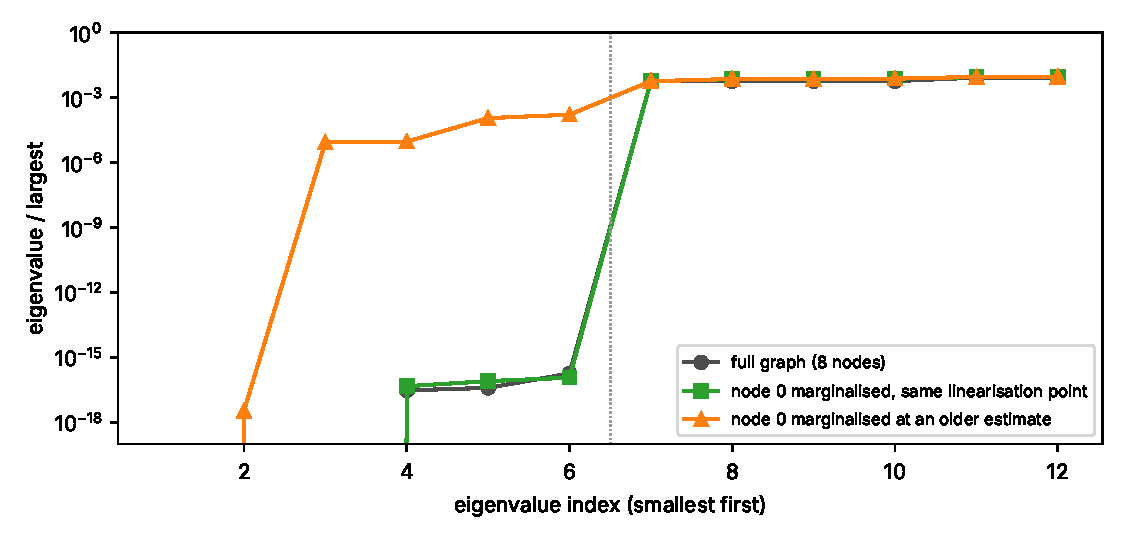
\includegraphics[width=0.8\linewidth]{figures/ch09_fej.pdf}
\caption{Smallest eigenvalues of the information matrix of an 8-node
pose graph with no fixed node (6 zero eigenvalues: the gauge), and after
marginalising node~0, with its factors linearised either at the current
estimate (the gauge survives) or at an estimate perturbed by about
5\,cm and $3^\circ$ (four spurious eigenvalues appear).}
\label{fig:fej}
\end{figure}

\section{Incremental smoothing}

Re-solving a pose graph after each loop closure is cheap; re-solving a
full factor graph with tens of thousands of variables after each frame
is not. iSAM2 (Kaess et al., 2012) keeps the factorisation of the
information matrix, organised as a \emph{Bayes tree} --- a tree of
cliques obtained from variable elimination --- and, when new factors
arrive, re-eliminates only the part of the tree they affect;
variables whose estimates moved by more than a threshold are
relinearised (``fluid relinearisation''), the rest keep their
linearisation point. Most updates touch only the top of the tree, and
the cost per step stays nearly constant, while a loop closure re-solves
the loop. GTSAM's \code{ISAM2} class implements it; we do not reimplement
it here, but every ingredient --- elimination, fill-in, marginalisation,
relinearisation --- is in this and the previous chapters.

\begin{mower}
For the PG98~HK the plan is now complete enough to sketch: the VO with
local BA runs in real time; every keyframe enters a pose graph; when a
loop closure is detected (next chapter), the pose graph is re-optimised
in a background thread with a robust kernel, and the local map is moved
with it. The mowing pattern helps: every row sees the same fence, house
and trees as its neighbours, so loops come often and early. And the pose
graph is also where the satellites will enter: an RTK-GNSS fix is just
one more factor --- a unary factor on a single pose --- added to the
same graph in Chapter~14.
\end{mower}

\begin{practice}[\code{vslam/posegraph.py}, \code{vslam/lie.py},
  \code{examples/ch09\_posegraph.py}, \code{notebooks/ch09\_posegraph.ipynb}]
\begin{center}
\begin{tabular}{@{}ll@{}}
\toprule
Code & Formula\\
\midrule
\code{lie.se3\_ad}, \code{se3\_right\_jacobian}, \code{\_inv} &
  \cref{thm:jrse3}\\
\code{posegraph.edge\_residual}, \code{edge\_jacobians} &
  \cref{prop:between}\\
\code{posegraph.PoseGraphProblem} & \cref{def:posegraph}, for
  \code{vslam.optim}\\
\code{posegraph.odometry\_edges}, \code{covisible\_loops} & building the
  graph\\
\code{posegraph.marginalize} & \cref{prop:margprior}\\
\bottomrule
\end{tabular}
\end{center}
The tests check the $\SE3$ Jacobian and its inverse against finite
differences, $\ad$ against the commutator, the factor Jacobians, exact
recovery of a noise-free graph, the 6-dimensional gauge without a fixed
node, a loop closure removing most of the drift of a biased odometry
around a square, a Cauchy kernel surviving a wrong loop that ruins least
squares, and marginalisation against the joint covariance. The notebook
also shows the effect of the odometry noise model and of overconfidence
on robust estimation.
\end{practice}

\section*{Further reading and C++ pointers}
\addcontentsline{toc}{section}{Further reading and C++ pointers}

F.~Dellaert and M.~Kaess, \emph{Factor Graphs for Robot Perception},
2017; M.~Kaess et al., ``iSAM2: incremental smoothing and mapping using
the Bayes tree'', IJRR 2012; G.~Grisetti, R.~K\"ummerle, C.~Stachniss and
W.~Burgard, ``A tutorial on graph-based SLAM'', 2010; N.~S\"underhauf and
P.~Protzel, ``Switchable constraints for robust pose graph SLAM'', IROS
2012; P.~Agarwal et al., ``Robust map optimization using dynamic
covariance scaling'', ICRA 2013; H.~Yang, P.~Antonante, V.~Tzoumas and
L.~Carlone, ``Graduated non-convexity for robust spatial perception'',
RA-L 2020; G.~P.~Huang, A.~I.~Mourikis and S.~I.~Roumeliotis, on
first-estimate Jacobians and observability (ISER 2008, IJRR 2010). In
C++: GTSAM (\code{BetweenFactor<Pose3>}, \code{ISAM2}), g2o
(\code{EdgeSE3}), Ceres with a \code{Manifold} for $\SE3$.

\FloatBarrier
\section*{Exercises}
\addcontentsline{toc}{section}{Exercises}

\begin{enumerate}[label=\textbf{9.\arabic*},ref=9.\arabic*]
\item\label{ex:9tree} Show that if a pose graph has no loops (it is a
  tree), its optimum fits every factor exactly: all residuals are zero.
  What does this say about odometry alone?
\item\label{ex:9linear} Show that for a factor graph whose residuals are
  affine in the variables, the linearisation point of a marginal prior
  does not matter. Why, then, is \cref{prop:fej} a phenomenon of
  nonlinear estimation only?
\item\label{ex:9loss} List what is lost when a bundle adjustment is
  replaced by a pose graph with one factor per pair of consecutive
  keyframes.
\item\label{ex:9ad} Compute the eigenvalues of $\ad\bxi$ and explain why
  the series for $J_r^{-1}$ diverges when $\norm{\bphi}\ge2\pi$.
\end{enumerate}

\subsection*{Solutions}

\textbf{9.1.} Root the tree at the fixed pose. Visit the nodes in
breadth-first order and set each child to $T_j=T_iZ_{ij}$ (or
$T_i=T_jZ_{ij}^{-1}$ when the edge points the other way): every factor
is then satisfied exactly, the cost is zero, and zero is the minimum of a
sum of squares. Odometry alone, a chain, is therefore never corrected by
optimisation: only loops create redundancy, and redundancy is what an
optimiser averages.

\textbf{9.2.} With affine residuals, every Jacobian is constant, so the
normal equations of the removed factors, hence $H'$, do not depend on
where they are evaluated, and $\vect{g}'$ is affine in the estimate in a
way consistent with the remaining factors (it is the exact marginal of a
Gaussian). The null spaces of all Jacobians coincide. In nonlinear
problems the null space $N(\btheta)$ of the gauge depends on $\btheta$
--- for example the direction of a global rotation about the origin acts
differently on poses at different positions --- and so does each
Jacobian.

\textbf{9.3.} The 3D points and the fact that a point seen by many
keyframes couples all of them (the marginal on the keyframes is dense on
covisible sets, not a chain); the non-Gaussian, non-linear shape of that
marginal; the possibility to relinearise the measurements as the
estimates move; and the ability to recompute the map consistently. The
pose graph keeps a Gaussian summary of each consecutive pair, linearised
once.

\textbf{9.4.} $\ad\bxi$ is block triangular with diagonal blocks
$\hatop{\bphi}$, so its eigenvalues are those of $\hatop{\bphi}$, each
twice: $0$ and $\pm i\norm{\bphi}$. The series $\sum B_nz^n/n!$ has
radius of convergence $2\pi$ (the nearest singularities of $z/(e^z-1)$
are at $\pm2\pi i$), and a matrix power series converges when the
spectral radius is within the radius of convergence; at
$\norm{\bphi}\ge2\pi$ it is not. Geometrically, $J_r$ is then singular:
the exponential map is not locally invertible there.
